%-----------------------------------------
%
\section{Performance Degradation}
\label{performance-analysis}
%
%-------------------------------------------

The Performance Degradation concept for set-point and
load-disturbance tunings depending on the operation mode was
previously presented and developed in \cite{arrietaCSC2007} and it
is succinctly reproduced here for sake of completeness and because
it is important to have a clear idea of how is defined and
computed. There, the performance of the control system is measured
in terms of a performance index that takes into account the
possibility of an operation mode different from the selected one.
This motivates the redefinition of the ISE performance index as

\be J_x(z)=\int_0^{\infty} e(t,x,z)^2 dt
\label{generic_index_operating_mode} \ee

\noindent where $x$ denotes the \emph{operating mode} of the
control system and $z$ the selected operating mode for tuning,
i.e., the \emph{tuning mode}. Thus, we have $x \in
\left\{sp,ld\right\}$ and $z \in \left\{sp,ld\right\}$, where $sp$
states for set-point (servo) tuning and $ld$ for load-disturbance
(regulator) tuning. Obviously, for one specific process it has to
be verified that

\bea J_{sp}(sp) & \leq & J_{sp}(ld) \nonumber\\
J_{ld}(ld) & \leq & J_{ld}(sp) \nonumber \eea

Performance will not be optimal for both situations. The
Performance Degradation measure helps in the evaluation of the
loss of performance with respect to their optimal value.
Performance Degradation, $PD_x(z)$, will be associated to the
\emph{tuning mode} - $z$ -  and tested on the, opposite,
\emph{operating mode} - $x$ -. According to this, the Performance
Degradation of the load-disturbance tuning, $PD_{sp}(ld)$, will be
defined as

\be PD_{sp}(ld) = \left | \frac{J_{sp}(ld)
-J_{sp}(sp)}{J_{sp}(sp)} \right | \label{PD_load_disturbance} \ee

\noindent whereas the Performance Degradation associated to the
set-point tuning, $PD_{ld}(sp)$, will be

\be PD_{ld}(sp) = \left | \frac{J_{ld}(sp)
-J_{ld}(ld)}{J_{ld}(ld)} \right |. \label{PD_set_point} \ee

Note that, because the controller settings expressed through
(\ref{set_point_tuning_formulae}) and
(\ref{load_disturbance_tuning_formulae}) have explicit dependence
on the process normalized dead-time $\tau$, it is worth taking
into account that, for the PID application, the Performance
Degradation will also depend on $\tau$. Fig. \ref{PerfDegradation}
shows the performance analysis for the normalized dead-time ranges
where PID controller settings are provided by
\cite{zhuangAthertonIEE1993}.

\begin{figure}[h!]
    \begin{center}
        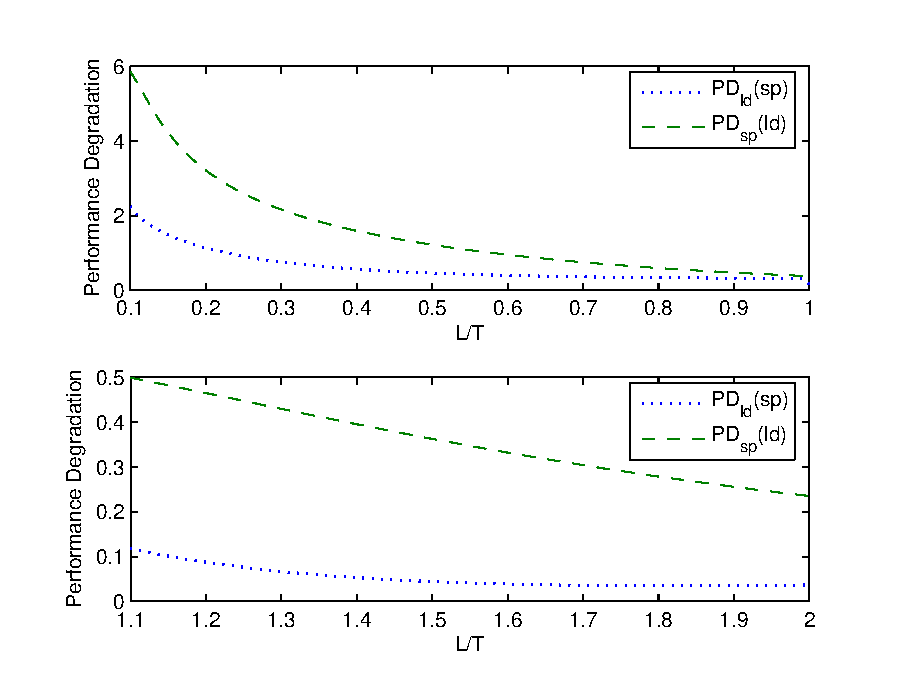
\includegraphics[width=0.8\linewidth]{PerfDeg.eps}
        \caption{Performance Degradation of set-point (sp) and load-disturbance (ld) tunings for ISE criteria with respect to the
        normalized dead-time $L/T$.}
        \label{PerfDegradation}
    \end{center}
\end{figure}

Note also that Performance Degradation is a decreasing function of
the normalized dead-time, taking very high values for processes
with small normalized dead-time.

The final decision for the choice of the appropriate tuning mode
will depend on the preference or importance that is given for the
system operation as regulator or as servo. However, if both
situations are likely to occur, Fig. \ref{PerfDegradation}
suggests a set-point based tuning is to be preferred, because it
provides lower Performance Degradation than load-disturbance
tuning.
